\chapter{Die Ethik im Bereich der KI}
\label{chap:Die Ethik }

\begin{figure}[h]
    \centering
    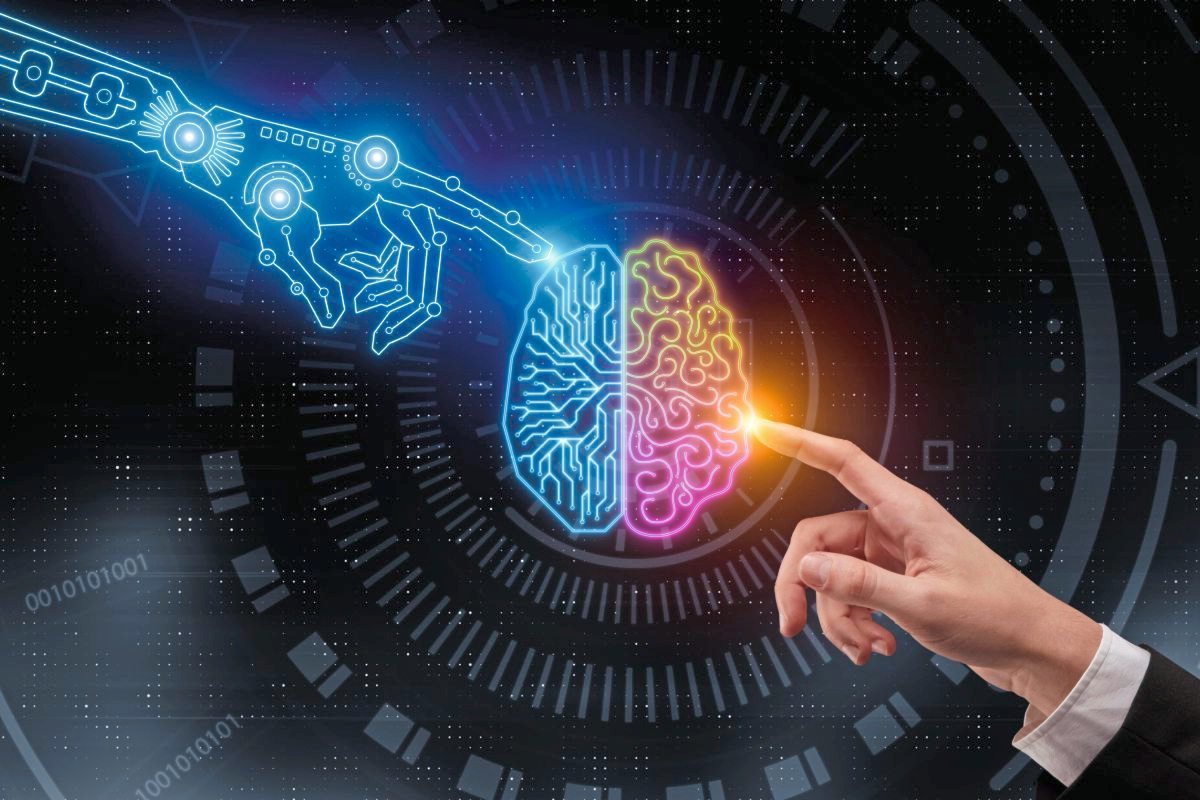
\includegraphics[width=0.5\textwidth]{KI4.jpg} 
    \caption{Die Ethik}
    \label{fig:ai}
\end{figure}

Die Ethik im Bereich der KI bezieht sich auf verschiedene Bereiche, darunter die Rolle der KI in der Gesellschaft und die ethischen Werte. Ein wichtiger Aspekt der KI ist das ethische Verhalten der Maschinen, der Einsatz muss den Grundsätzen der Rechtmässigkeit, Transparenz, Sicherheit und Verantwortlichkeit entsprechen. Die KI darf nie diskriminieren oder Vorurteile verstärken. Die Gestaltung der KI muss der Würde des Menschen und den Grundrechten entsprechen. Bevor dem Einsatz der KI müssen die Risiken bewertet werden, um potenzielle negative Auswirkungen zu erkennen und zu minimieren. Die Einhaltung ethischer Grundsätze ist im Bereich der KI von entscheidender Bedeutung, damit KI-Systeme verantwortungsbewusst eingesetzt werden.